\documentclass{article}
\usepackage[a4paper]{geometry}
\usepackage[utf8]{inputenc}
\usepackage{xurl}
\usepackage{graphbox}
\usepackage{graphicx}
\usepackage{pdflscape}
\usepackage{array}
\usepackage{caption}
\usepackage{hyperref}

\graphicspath{ {./imgs/} }

\title{The Evolutionary Exploration of Emergent Execution: AIMEE Progress Report}
\author{Francisco Blas Izquierdo Riera\footnote{This reflects only the autorship of this technical report describing the current status of the project and not the authorship of the contributions of the project. Francisco would like to note that his role in these contributions has been fairly small and that most of the work has been performed by other members of the team.} \\ (Special Circumstances Inc.)}
\date{December 2020}

\begin{document}

\maketitle

\tableofcontents

\listoffigures

\section{Introduction}

\subsection{Control flow takeover attacks}
In most systems it is common to have only a single memory that combines instructions, execution control data and program data.

Instructions specify the operations that the system has to execute, execution control data specify which instructions to run next and program data contain user inputs and any intermediate steps needed to produce the desired outputs.

Execution control data is usually implicit, meaning "execute the next instruction after this one"; but may be implicit in the instruction, for example, the address provided in a jump instruction indicating which instruction to execute next; or implicit in the control data memory, for example, a procedure return instruction extracting the instruction to execute next from the control data stack.

Certain kinds of attacks are the result of mixing instructions and program data in the same memory. Such attacks arise from programming errors. This can be because the programmer did not allocate memory sizes correctly, which an attacker can use to get the system to overwrite legitimate instructions with their own that will be executed later. If the programmer did not properly segregate program data from program instructions, an attacker could use this to alter the program data with the aim of confusing the system to use the program data as part of the instruction flow. Two clear examples of this second case are SQL Injection and Cross-Site Scripting attacks. 

In a similar way, control flow takeover attacks are attacks arising from a bug that makes the system confuse program data with control flow data. The most common example happens when data written to a buffer allocated on the, common, stack overwrites control flow data like the return address, making the program continue execution on a different place. Attacks can be triggered in different ways. An error that leads to "confusion" between different data structures can be used by an attacker to overwrite control data allowing them to send the program flow to a memory address under the attacker's control. Similarly, other programming errors can let an attacker overwrite the control data containing addresses to external libraries. This attack will result in the attacker's libraries or functions being called instead of the addresses contained in the original program.

\subsection{History of Return Oriented Programming}
Historically, control flow takeover attacks exploited also the mixing of instructions and program data. In particular, the attacker introduced the code to be ran, known as shellcode, as part of the data and then tried to redirect the program flow into the instructions in said buffer.

Over time different measures appeared to make such attacks harder.

By allocating the buffer at a non deterministic position (for example by changing the addresses used by the memory regions of the program) the attacker had to figure out the right address at which the buffer was found. To address this, attackers usually introduced large sequences of instructions performing no changes (no operations or NOPs) so that their guessed address would hopefully fall somewhere in that instruction list. These sequences of instructions are known as NOP-sleds since it is expected that once in them the program flow will slide gracefully towards the shellcode.

An additional measure implemented when such issues occurred on the stack was the introduction of canaries. Canaries are little pieces of data introduced before the return address and programmatically compared to their original value before reading the return address.  Canaries can be effective in some cases when the attacker's code overwrites the memory occupied by the canary and while having no way of knowing their value in advance. They are less effective when the attack is more stochastic and could leave them intact after the attack. A canary can also be evaded when its value remains the same over time, allowing the attacker to overwrite them with their original value during each attack attempt to prevent triggering the security measure. 

Another, very effective, measure against such attacks was the introduction of memory markings. Memory markings indicate the operations that can be performed on a specific chunk of memory and are, generally, in a different area of memory than program memory (often requiring kernel level privileges to modify). The permissions in such memory chunks are commonly reading (which is frequently implicitly granted by allowing access to the memory), executing (interpreting the memory as code) and writing (modifying the memory contents).

As a consequence of memory markings, modern software distinguishes between program data and instructions (and when performing JIT the intersection of both). In particular, this  entails that most of the control data that does not need to be modified in the future can be marked as read-only (for example function pointers to shared libraries) once it has the desired value. This makes control flow attacks on these impossible. Similarly,
the stack containing control flow and program data is usually marked not executable preventing the attacker from executing code loaded on the stack.

Still the issue of mixing control flow data and program data remains, although now, the attacker is limited in his ability to introduce code. In this context attackers started looking at executing already present code in a different order than originally intended. Under normal circunstances, such pieces of code would execute until the subroutine return instruction. This instruction, would read a value from the stack and continue execution on this value allowing composability of code sequences. Each such sequence of instructions is known as a gadget as it provides a limited set of side effects on the machine. The result of chaining the execution of such gadgets by queuing their address on the stack so they would be executed after each return is known as ROP (return oriented program) programming.

\subsection{Challenges of return oriented programming}
Return oriented programming presents a large set of challenges. Identifying and recognizing useful gadgets is a difficult task even for humans to perform. Composing them into meaningful ways while keeping their side effects under control is even more complicated.

For example, to be able to run an existing program inside the system, the attacker needs to be able to load the desired values on the registers and then execute the instruction sequence to trigger a request to the operating system. Being able to read and write from arbitrary memory addresses may entail finding instruction sequences that allow an attacker to figure out the target address to impact and then write the desired value to an attacker controlled address.

Due to all this complexity the Berbalang project aims at using genetic algorithms to create diverse populations of composable gadget sequences that can trigger desirable outcomes. This is done assuming the attacker has control of the stack at a specific point of execution and evolving different buffers that emulate the contents of such an attack. Unlike the original ROPER developed by Olivia Lucca Fraser which focuses on finding specific solutions satisfying certain criteria. Berbalang has a focus on finding a larger variety of program populations providing different interesting solutions so that the results convey a certain measure of the attacker's ability to reuse code for such attacks.

\subsection{Genetic algorithm concepts}
Genetic algorithms work on an idea similar to that in which living organisms evolve. Each candidate is represented by a small sequence of data (genotype) which after running a specific process produces an output (phenotype). Using some scoring of the resulting outputs a selection of the best candidates is made.

Successful candidates are replicated but, for the algorithm to progress, certain changes need to be introduced into said candidates. These are done using different genetic operators which change a candidate's genotype (mutation) or combines the genotypes of two candidates (crossover).

Crossover can be performed in different manners. A common choice is concatenating the genotype of a candidate to another one at a specific point (single point crossover). Another common choice is interleaving elements from the genotype of one candidate with those of the other (alternating crossover).

Candidates may be isolated in different populations that interact in selection processes in different ways. This is known as geography.

\section{Addressing the challenges of return oriented programming}
As longer instruction sequences are evaluated, the amount of side-effects introduced grows linearly. Similarly, when composing instruction sequences, longer compositions introduce more side-effects.

Trying to find good gadgets and composing them into meaningful chains requires being able to reason about these side-effects. This task is already hard to perform for humans and is likely also complex for computer systems. Among the reasons of this complexity is the fact that heuristics used to find a solution, that humans have in the form of intuition, can be hard to define or model.

Instead, genetic algorithms look promising as a way to find solutions that have desirable properties. Properties like, for example: length; amount of side effects; or control over such effects.

Genetic algorithms also offer the advantage of being able to avoid thinking about the individual consequences of the side-effects of each instruction and their compatibility. Instead, they can focus only on the final results caused by the combination of all of the side-effects. Because of this, such algorithms are a very promising tool for finding solutions to problems like having control of a processor's registers. On the other hand, developing metrics based on the composability and level of control allowed by a specific set of gadgets is a bit more complex and requires choosing those that would maximize the desired effects while giving enough space for evolution and novelty to avoid getting stuck in local maxima.

\section{Genetic algorithm choices}
In the following sections we describe the different choices that were made regarding the genetic algorithm for the experiments performed. These choices were made not only with the objective of generating desirable solutions but also with the idea of improving population variability.

\subsection{Genotypes}
As we mentioned earlier, the genotype defines the kind of input that is given to the evaluation program. To that matter we considered two different possibilities:
\begin{enumerate}
    \item Arrays of integers
    \item Payload builder instructions
\end{enumerate}

An array of integers is the simplest way of modeling such a problem. If the integers have the size of a processor word, they would represent either: addresses on which to run code, or data to be used by the code (for example to load on registers). This is a very simple concept to work with and also directly models the payload that the attacker would introduce with an attack. The main issues of this approach is that it lacks any context or information about the meaning of the different integers which can be problematic for example when using certain genetic operators.

A second option is to use a set of instructions that explain how to build the desired payload. This is more advanced but allows, for example, building programs which are aware of the memory state on which the attack is emulated. In our case this also made possible using Falcon for semantic analysis and to design a virtual machine providing a higher level interpretation of the stack for modelling execution.

The project moved from the first kind of representation to the second.

\subsection{Phenotypes}
When running our payloads, we can note the observed behavior on execution including a possible mapping of the results to the ROP payload contents. To obtain a fitness value we then apply functions to map these behavior patterns modelling different execution profiles into arrays of scalar values. Finally we add them with weights to obtain the targeted fitness value.

Since we also try to target the composability of the different chains to get a meaningful combination of gadgets we also take into account only those populations that can arrive to a commitment point. In the experiments we have considered this point to be ending the execution with an empty stack and thus making use of all the payload data. To handle this correctly Berbalang keeps a log of the changes made by the program which are only taken into account once the commitment point is reached.

\subsection{Selection}
The project has considered different selection techniques:
\begin{enumerate}
    \item Roulette
    \item Pareto front
    \item Lexicase
    \item Tournament
\end{enumerate}

Of these tournament selection is seen as the most appropriate for the project. In Berbalang, this is implemented by choosing a group of contestants randomly on each iteration. In particular, 5 contestants are chose. Then the best are kept and bred. In our case we pick the best 2. Finally, the resulting offspring replaces those that performed worst in the comparison.

This selection process also allows to model different geographies when modeling populations to increase diversity and avoid local maxima.

\subsection{Geography}
In Berbalang we have tested an island geography with linear inner geographies.

Island geographies provide many advantages. Islands are usually handled independently having their own populations. Since islands are mostly isolated between them, parallelization of the algorithm is significantly simpler. This isolation also helps foster diversity as the best performers in a population will not always impact those on other islands. 

In order to ensure islands are not completely isolated, islands may use a shared "pier" to send or receive individuals at random intervals. In Berbalang this is modeled using a lockless queue.

Inside each island Berbalang operates making use of linear geographies. Each island contains a circular buffer meaning that all elements have a right and a left neighbor. Then the first contestant is picked up randomly from the buffer and any other contestants are picked randomly from those neighbors which are $n$ steps apart from the chosen contestant. This model allows keeping certain local variability in the population as changes may take various generations to reach populations which are further away. If such a behaviour is not desirable, all that is needed is making $n$ equal to the size of the circular buffer so that all members of the buffer can be chosen.

\subsection{Genetic operators}
Berbalang makes use of three types of genetic operators: alternating crossover of candidates, single point crossover and mutation.

\subsubsection{Alternating crossover}
When performing alternating crossover we merge together pieces alternating between both of their parents picking lengths from an exponential distribution (to favor shorter bits over longer ones). This approach prevents genetic bloat by ensuring childs have the same length their parents had.

\subsubsection{Single point crossover}
In this approach we pick a cut point on each of the parents and then concatenate the results. This approach is fairly efficient at implementation time but prevents intertwining composable gadgets.

\subsubsection{Mutation}
Finally children may also be subject to mutation, we perform this with a variety of operators. The first one entails applying bitwise operations to integers, these ensure that the children explore the available program and input space as desired. The second entails looking for references in memory containing the desired value and replacing the value with the address where it is placed in memory. Finally we have an operator that does the opposite replacing the value with the contents of the memory address at which it points.

Although these operators may appear fairly simple they allow to emulate the behaviour of other gadget programs and help ensure the algorithm covers different positions.

\section{Technical obstacles}
During the development of Berbalang we have found two main technical obstacles. Race conditions triggering strange behavior in Unicorn, the library used to run the code when testing populations; and CPU scalability issues affecting the performance of the system.

\subsection{Race conditions}
During experimentation, we found that parallel instances of Berbalang produced crashes. Research on the issue lead to writes into a structure which was pointing to NULL (an invalid address used to show a pointer points to nowhere).

After some tests the issue was pinpointed to a race condition between the main thread and the timeout callbacks which resulted in one setting the address to NULL before the other tried to access it. This was solved by synchronizing the accesses using a mutex so that only one of them would try to access the data at a time.

\subsection{CPU scalability}
After addressing this issue we found that the system had difficulties scaling to run on more than 5 cores. This can be seen on the usage graphics in figures \ref{fig:g1} and \ref{fig:g2}. Time limitations prevented fully delving into the issues causing this. Preliminary analysis shows that enough workers were waiting for execution. Memory or I/O pressure are considered the most likely causes behind these issues.

Further investigation on these issues may be performed if further development of Berbalang is performed as part of the project.

\begin{figure}[ht]
\centering
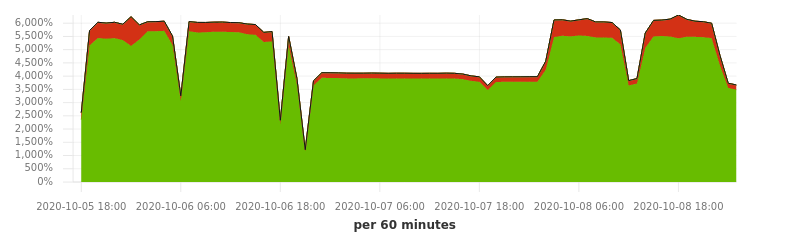
\includegraphics[width=\textwidth]{g1}
\caption{Percentage of CPU usage on AMD nodes}
\label{fig:g1}
\end{figure}
\begin{figure}[ht]
\centering
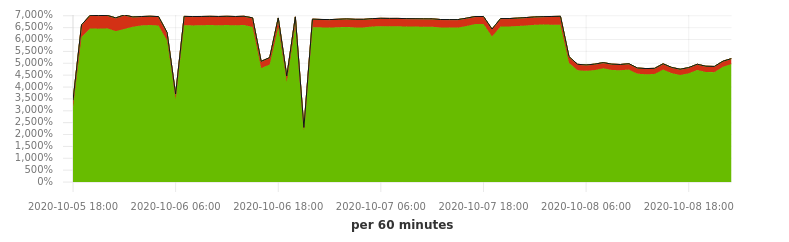
\includegraphics[width=\textwidth]{g2}
\caption{Percentage of CPU usage on Intel nodes}
\label{fig:g2}
\end{figure}

\section{Experiments}
During the experiments we tested different approaches for reproduction and for creating the initial populations. For crossover we tested purely asexual reproduction, applying the genetic operators only to create mutations, alternating crossover and single-point crossover. For the initial seeding of populations we tried both random initial values and values extracted using ROPgadget.

We considered also various metrics: the number of procedure return instructions executed; the coverage of the code by the population; the circulation of alleles across the population; and the generational distribution.

The fitness function that was used on the experiments was the coverage of code.


\subsection{Return count results}
A total of four experiments were run. In the first three, the cross product of reproduction and initial techniques were tested. In the fourth a run over significantly more iterations was made using only random seeding but with all three reproduction techniques.

The results of the experiments can be seen at figures \ref{fig:rc/e1}, \ref{fig:rc/e2} and  \ref{fig:rc/e3} for the first three experiments and at figure \ref{fig:rc/el} for the last longer one. Keep in mind that in the last experiment graphs the axis are not to scale between each other.

From the results in these figures, it is easy to notice that the highest number of executed return instructions result from sexual reproduction using single point crossover. This is probably caused by alternating crossover being more likely to mix payloads containing data other than return addresses.

Similarly, using ROPgadget to seed the initial populations increases significantly the number of executed returns on the single point crossover and slightly on the alternating crossover cases. The lack of impact on the asexual reproduction population likely stems from the inability to combine the return generating instructions from both parents.

\newgeometry{top=5mm, bottom=5mm, right=5mm,left=5mm}
\pagestyle{empty}
\begin{landscape}
\begin{figure}[t]
\begin{center}
\begin{tabular}{c c c c}
    Seeding & Asexual reproduction & Alternating crossover & Single point crossover \\
    Random & 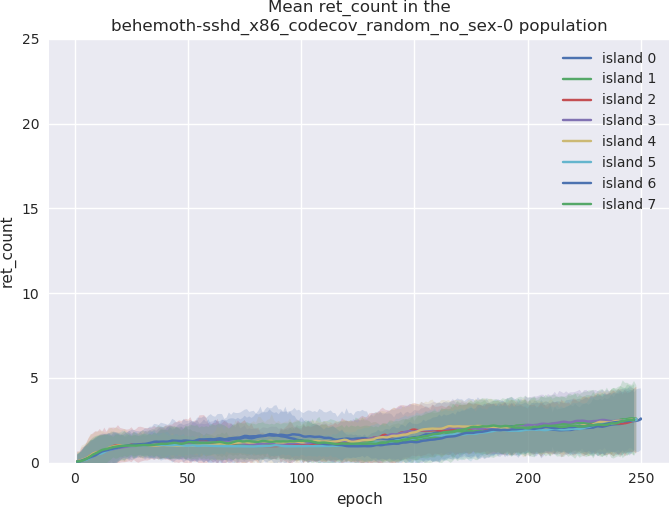
\includegraphics[align=c,width=0.42\textwidth]{rc/e1/1} & 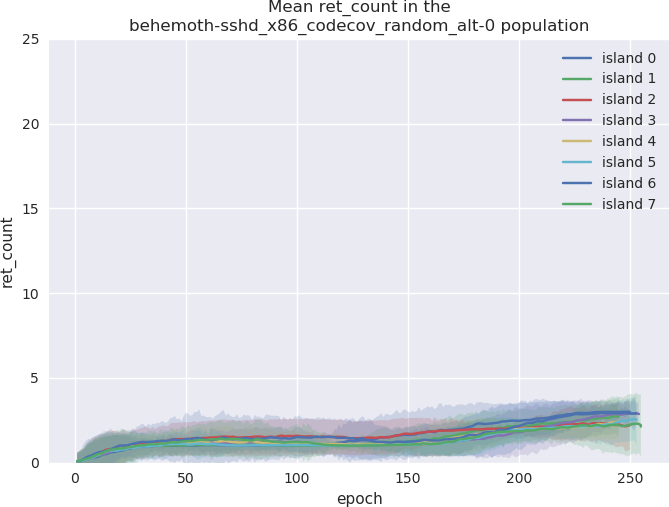
\includegraphics[align=c,width=0.42\textwidth]{rc/e1/2} & 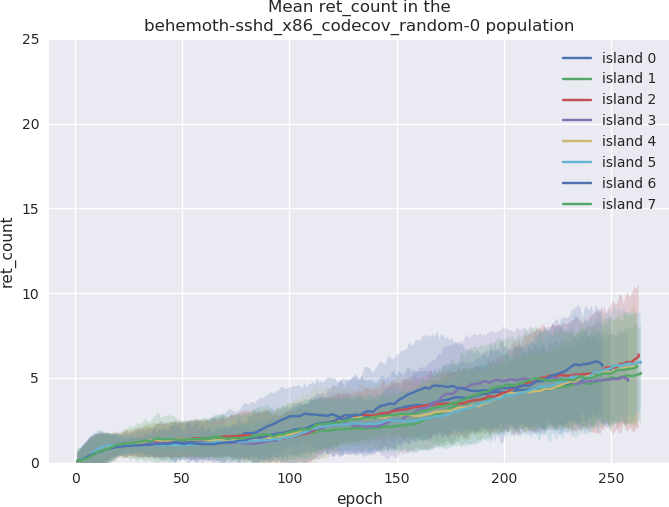
\includegraphics[align=c,width=0.42\textwidth]{rc/e1/3} \\
    & & & \\
    ROPgadget & 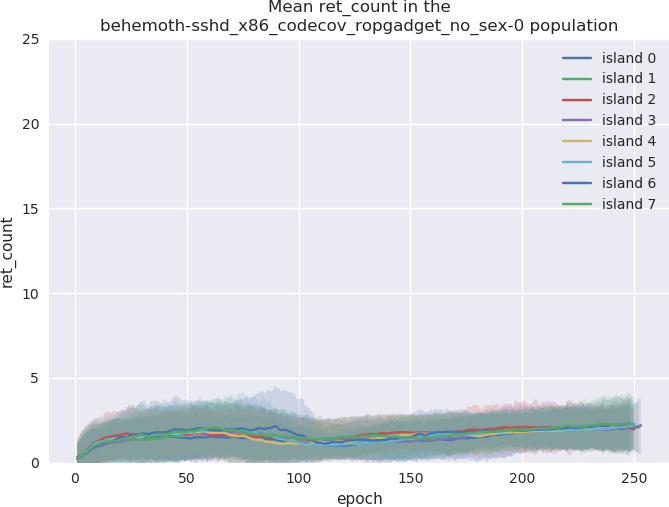
\includegraphics[align=c,width=0.42\textwidth]{rc/e1/4} & 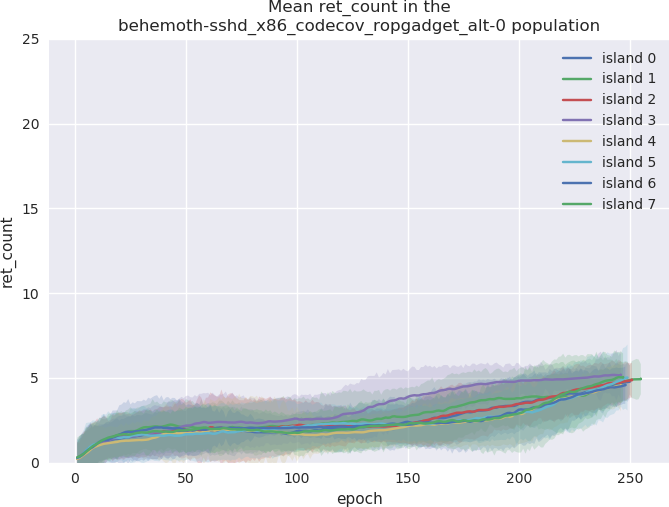
\includegraphics[align=c,width=0.42\textwidth]{rc/e1/5} & 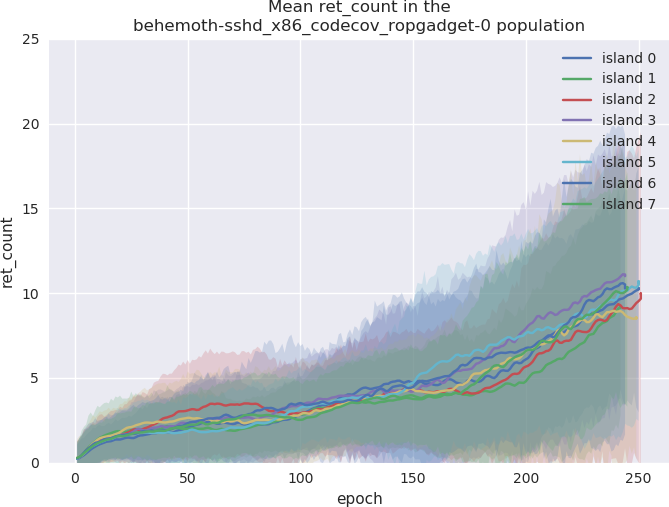
\includegraphics[align=c,width=0.42\textwidth]{rc/e1/6} \\
\end{tabular}
\end{center}
\caption{Return count of populations. Experiment 1.}
\label{fig:rc/e1}
\end{figure}

\begin{figure}[t]
\begin{center}
\begin{tabular}{c c c c}
    Seeding & Asexual reproduction & Alternating crossover & Fixed point crossover \\
    Random & 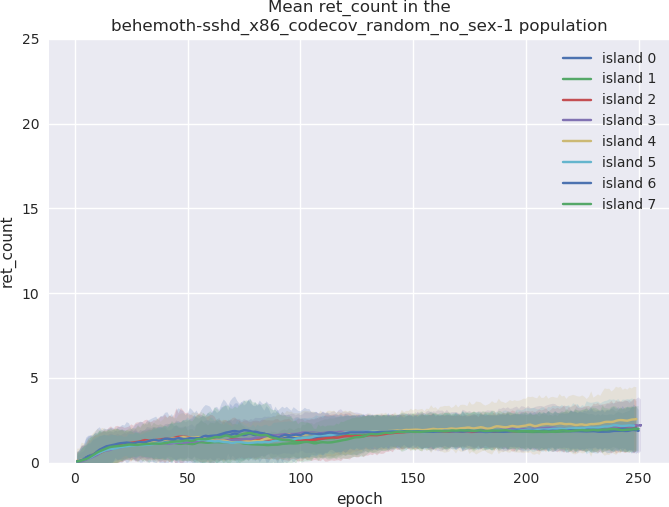
\includegraphics[align=c,width=0.42\textwidth]{rc/e2/1} & 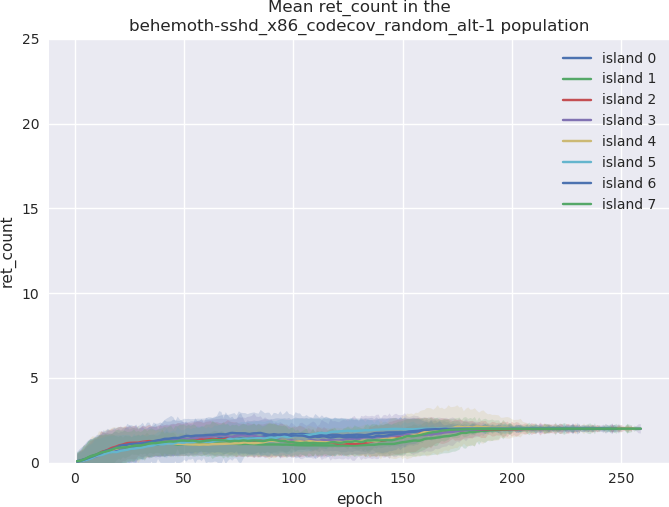
\includegraphics[align=c,width=0.42\textwidth]{rc/e2/2} & 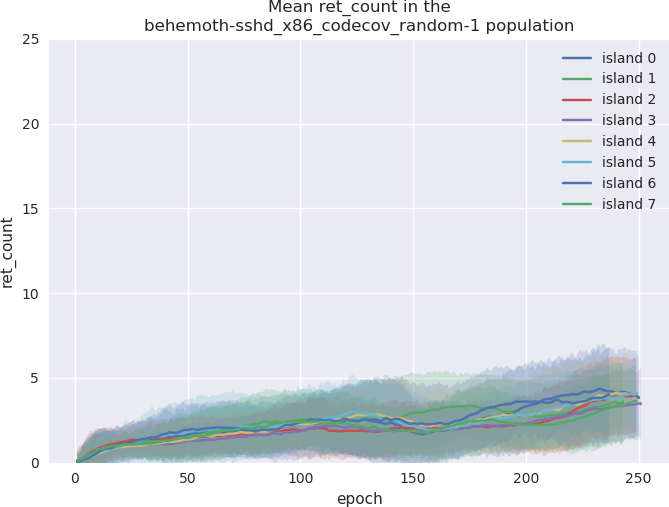
\includegraphics[align=c,width=0.42\textwidth]{rc/e2/3} \\
    & & & \\
    ROPgadget & 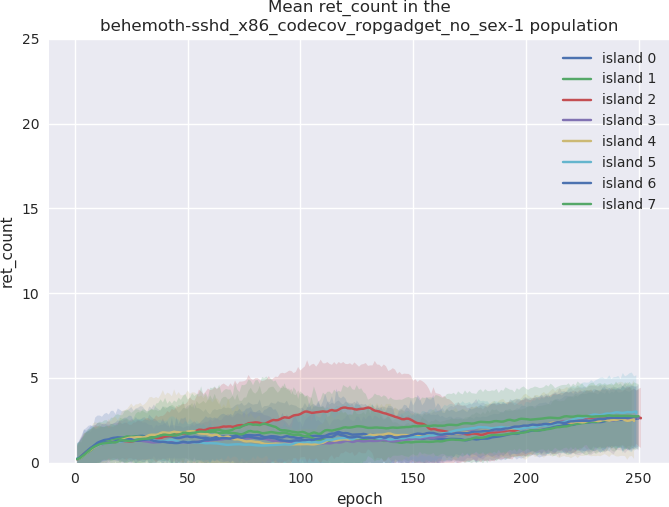
\includegraphics[align=c,width=0.42\textwidth]{rc/e2/4} & 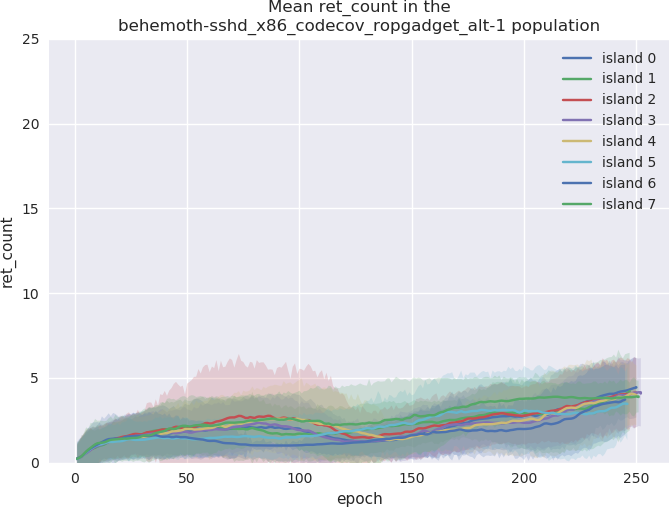
\includegraphics[align=c,width=0.42\textwidth]{rc/e2/5} & 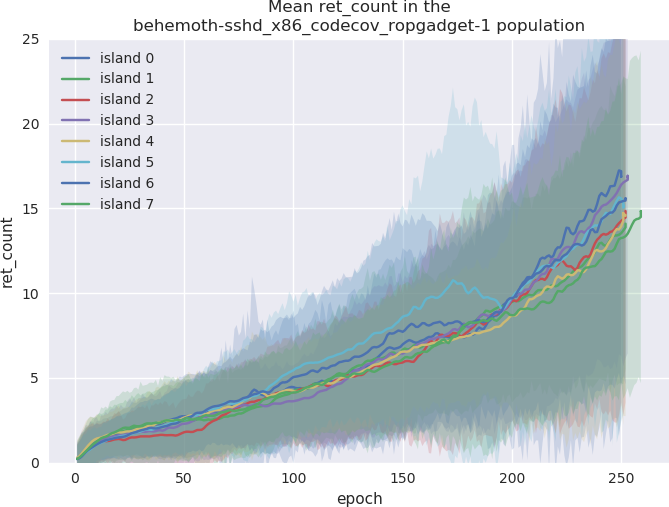
\includegraphics[align=c,width=0.42\textwidth]{rc/e2/6} \\
\end{tabular}
\end{center}
\caption{Return count of populations. Experiment 2.}
\label{fig:rc/e2}
\end{figure}

\begin{figure}[t]
\begin{center}
\begin{tabular}{c c c c}
    Seeding & Asexual reproduction & Alternating crossover & Fixed point crossover \\
    Random & 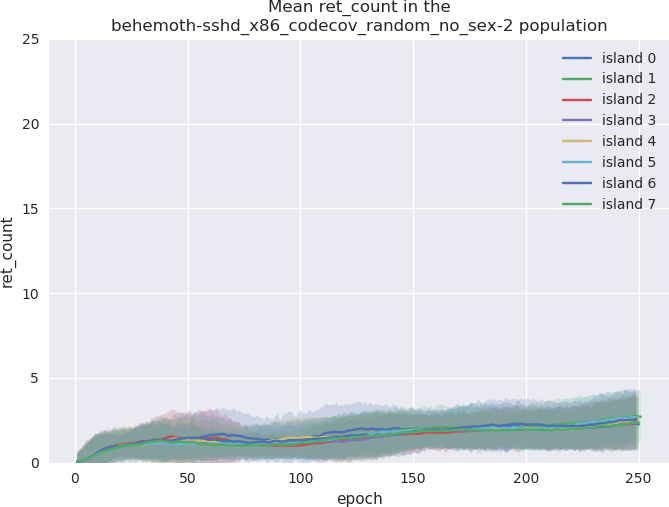
\includegraphics[align=c,width=0.42\textwidth]{rc/e3/1} & 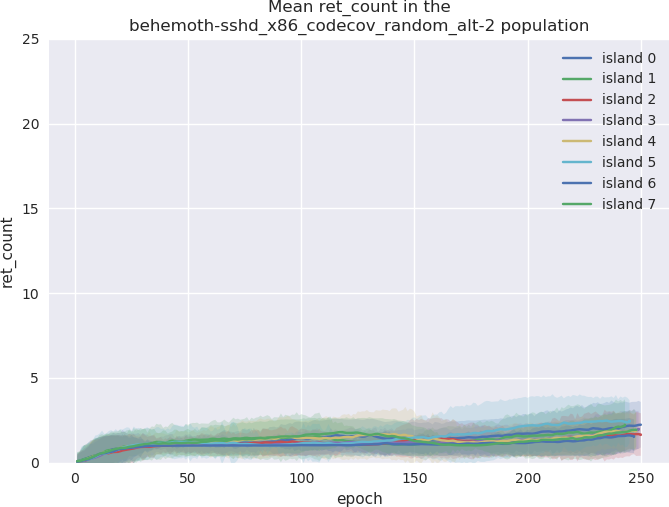
\includegraphics[align=c,width=0.42\textwidth]{rc/e3/2} & 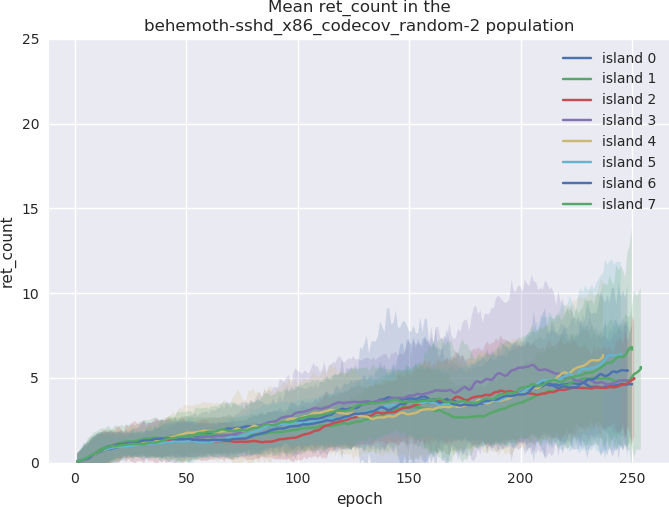
\includegraphics[align=c,width=0.42\textwidth]{rc/e3/3} \\
    & & & \\
    ROPgadget & 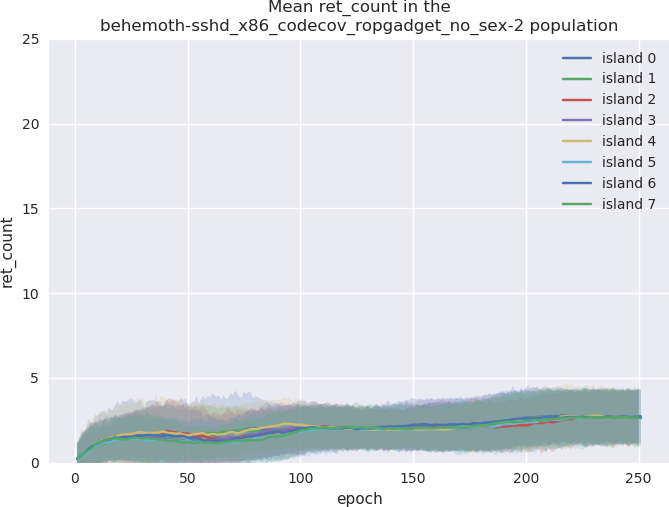
\includegraphics[align=c,width=0.42\textwidth]{rc/e3/4} & 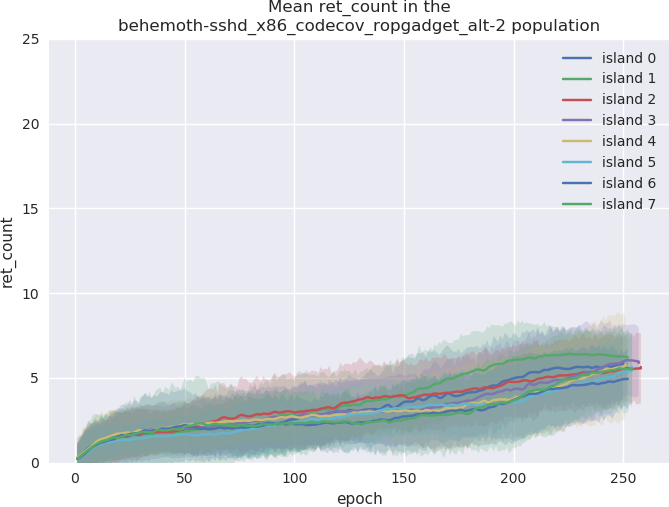
\includegraphics[align=c,width=0.42\textwidth]{rc/e3/5} & 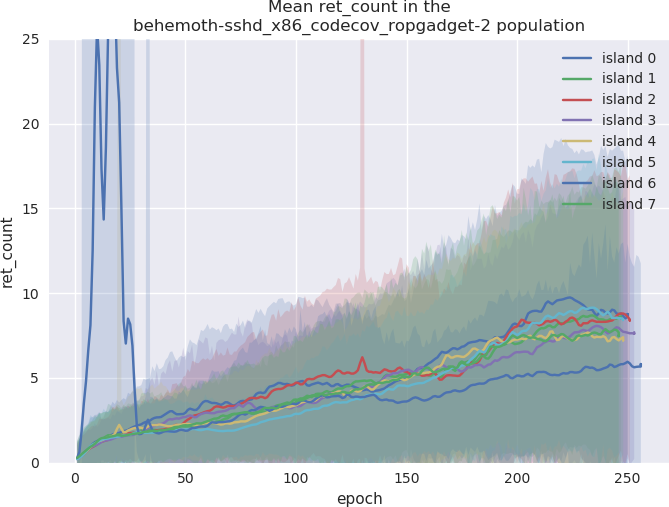
\includegraphics[align=c,width=0.42\textwidth]{rc/e3/6} \\
\end{tabular}
\end{center}
\caption{Return count of populations. Experiment 3.}
\label{fig:rc/e3}
\end{figure}

\begin{figure}[t]
\begin{center}
\begin{tabular}{c c c c}
    Seeding & Asexual reproduction & Alternating crossover & Fixed point crossover \\
    Random & 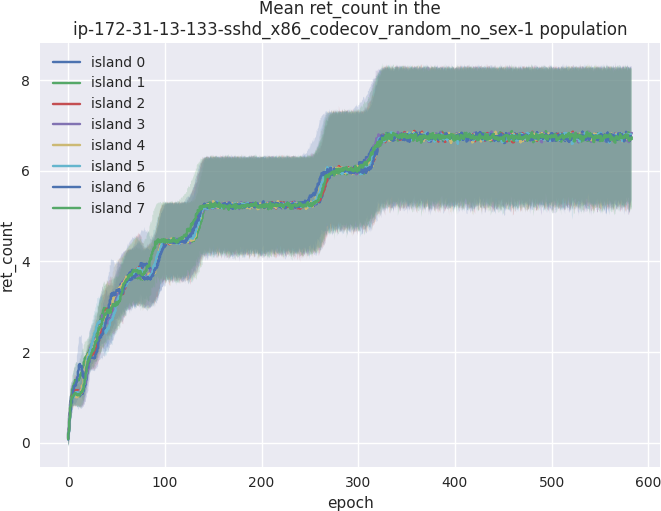
\includegraphics[align=c,width=0.42\textwidth]{rc/el/1} & 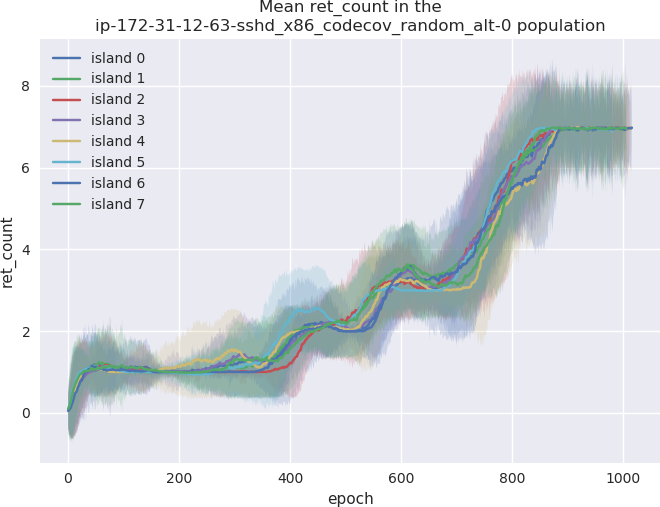
\includegraphics[align=c,width=0.42\textwidth]{rc/el/2} & 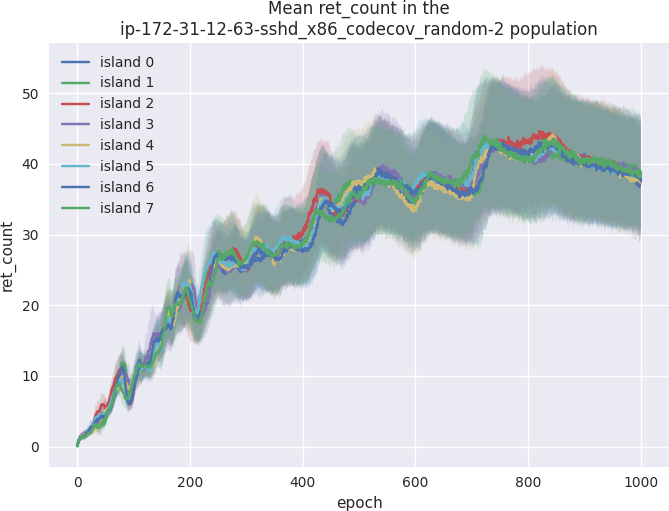
\includegraphics[align=c,width=0.42\textwidth]{rc/el/3} \\
\end{tabular}
\end{center}
\caption{Return count of populations. Experiment 4: longer runs over randomly seeded populations. Axis not to scale.}
\label{fig:rc/el}
\end{figure}
\end{landscape}
\restoregeometry
\pagestyle{plain}

\subsection{Code coverage results}
A total of three experiments were run. In all of them, the cross product of reproduction and initial techniques were tested. The results of the experiments can be seen at figures \ref{fig:cc/e1}, \ref{fig:cc/e2} and \ref{fig:cc/e3}.

From the results in these figures, it is easy to notice that code coverage was maximized by single point crossover reproduction. Asexual reproduction also consistently produced slightly better results than alternating crossover. This may be because of the issues with alternating crossover mentioned before.

Using ROPgadget had various effects. While in single point crossover reproduction this improved or maintained the code coverage, the results are less conclusive for the other two reproduction methods. This shows that the choice of a good reproduction method is significantly more important than a good initial seeding of the populations.

\newgeometry{top=5mm, bottom=5mm, right=5mm,left=5mm}
\pagestyle{empty}
\begin{landscape}
\begin{figure}[t]
\begin{center}
\begin{tabular}{c c c c}
    Seeding & Asexual reproduction & Alternating crossover & Single point crossover \\
    Random & 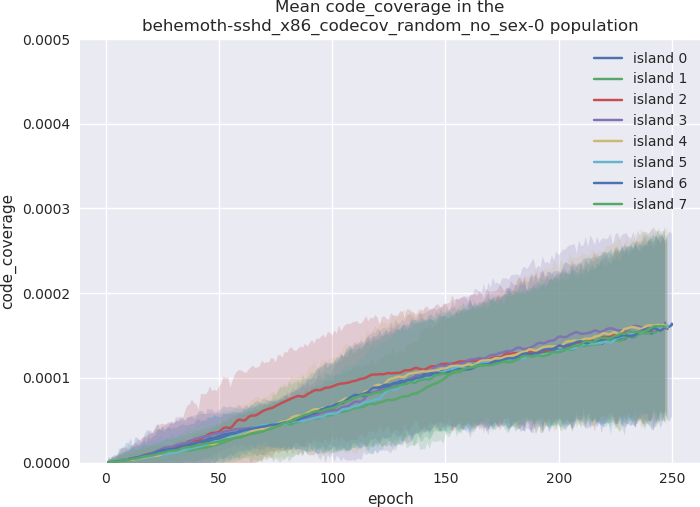
\includegraphics[align=c,width=0.42\textwidth]{cc/e1/1} & 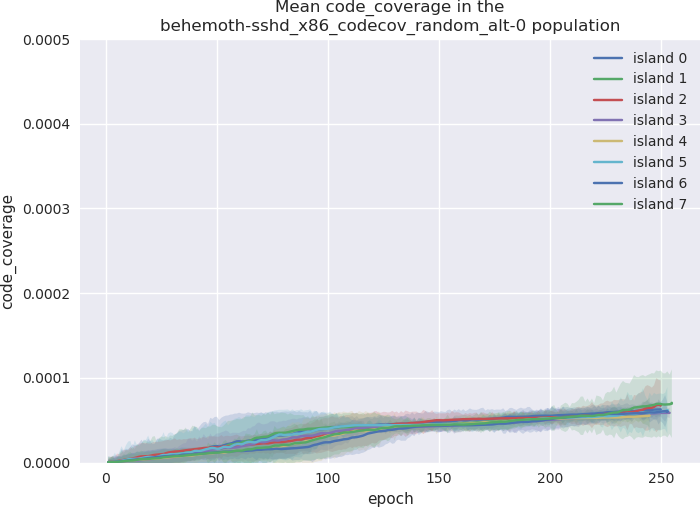
\includegraphics[align=c,width=0.42\textwidth]{cc/e1/2} & 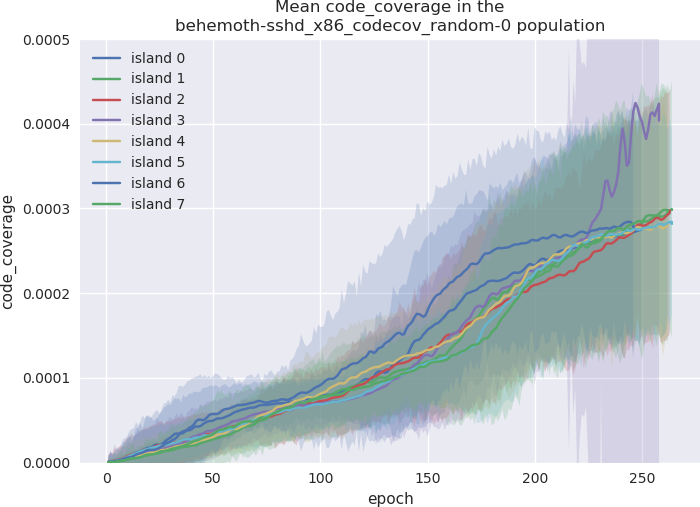
\includegraphics[align=c,width=0.42\textwidth]{cc/e1/3} \\
    & & & \\
    ROPgadget & 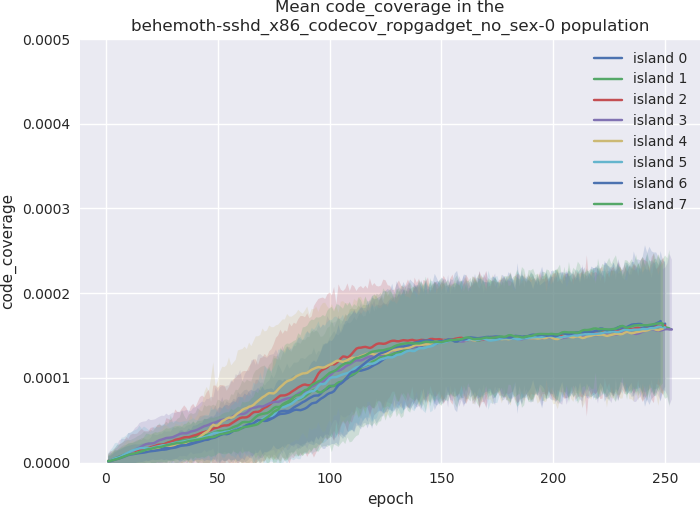
\includegraphics[align=c,width=0.42\textwidth]{cc/e1/4} & 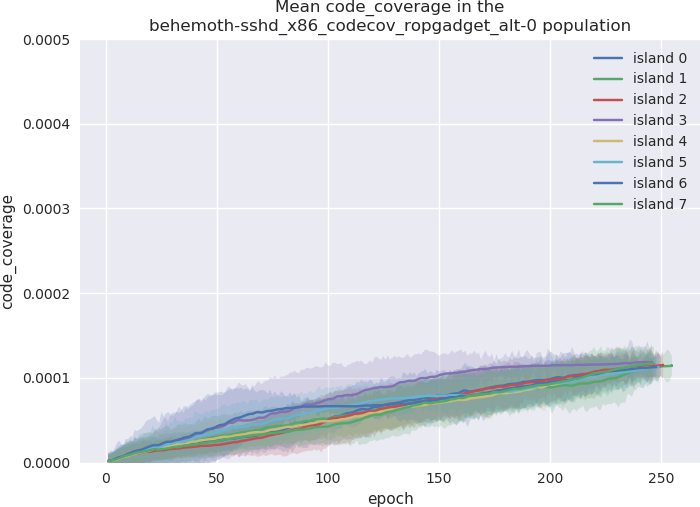
\includegraphics[align=c,width=0.42\textwidth]{cc/e1/5} & 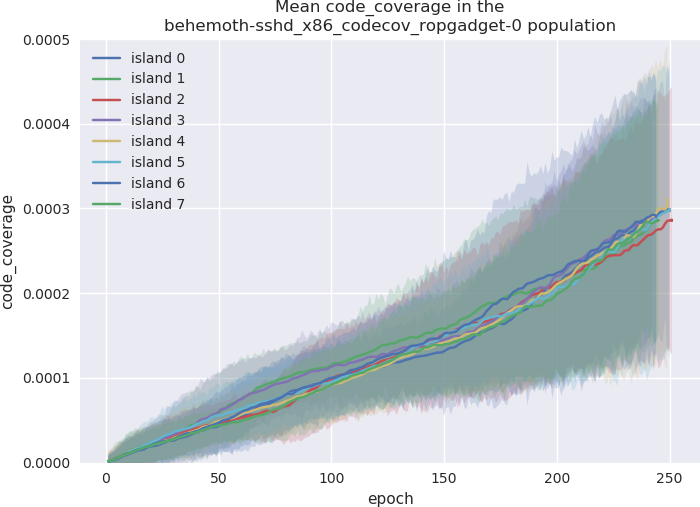
\includegraphics[align=c,width=0.42\textwidth]{cc/e1/6} \\
\end{tabular}
\end{center}
\caption{Code coverage of populations. Experiment 1.}
\label{fig:cc/e1}
\end{figure}

\begin{figure}[t]
\begin{center}
\begin{tabular}{c c c c}
    Seeding & Asexual reproduction & Alternating crossover & Fixed point crossover \\
    Random & 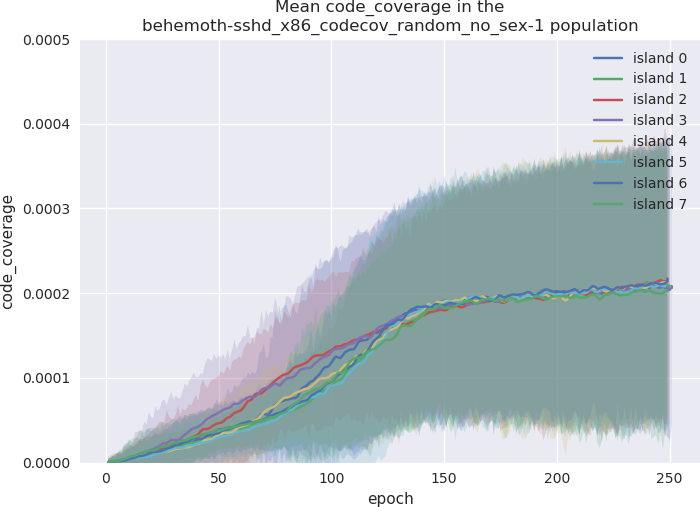
\includegraphics[align=c,width=0.42\textwidth]{cc/e2/1} & 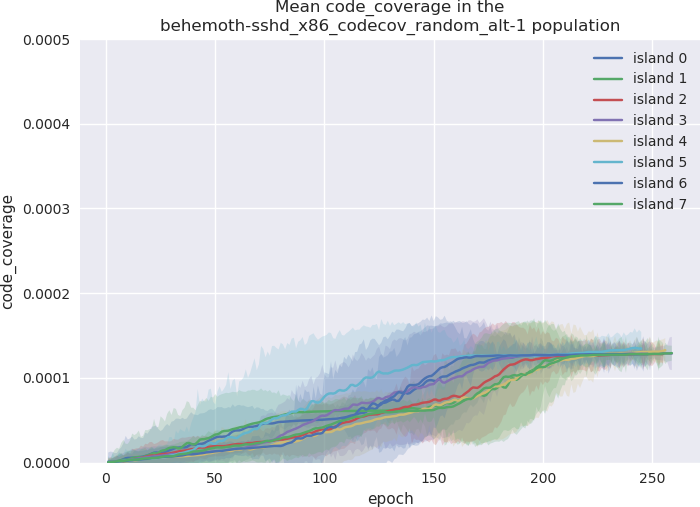
\includegraphics[align=c,width=0.42\textwidth]{cc/e2/2} & 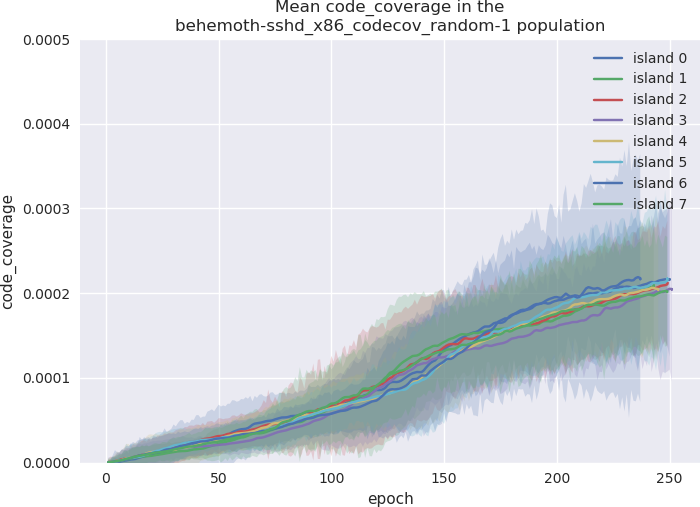
\includegraphics[align=c,width=0.42\textwidth]{cc/e2/3} \\
    & & & \\
    ROPgadget & 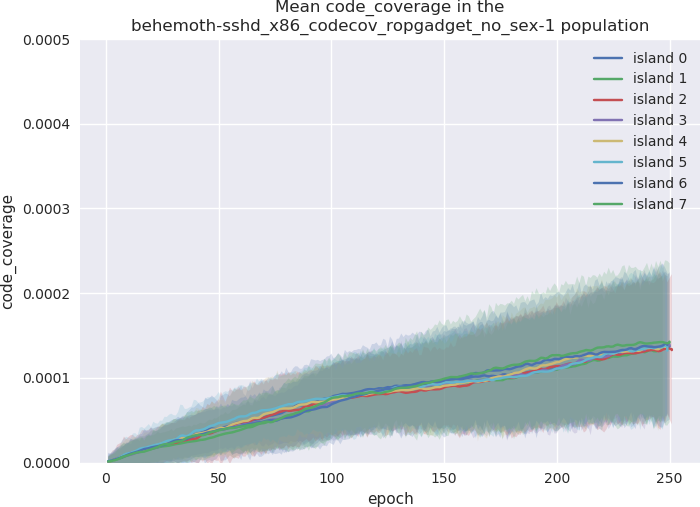
\includegraphics[align=c,width=0.42\textwidth]{cc/e2/4} & 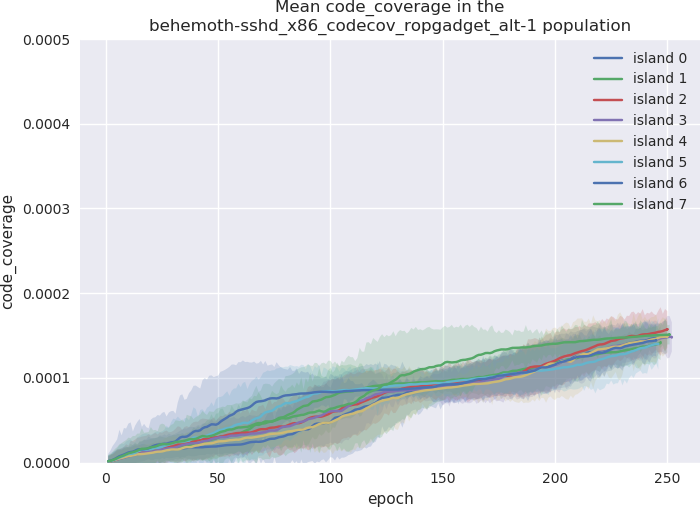
\includegraphics[align=c,width=0.42\textwidth]{cc/e2/5} & 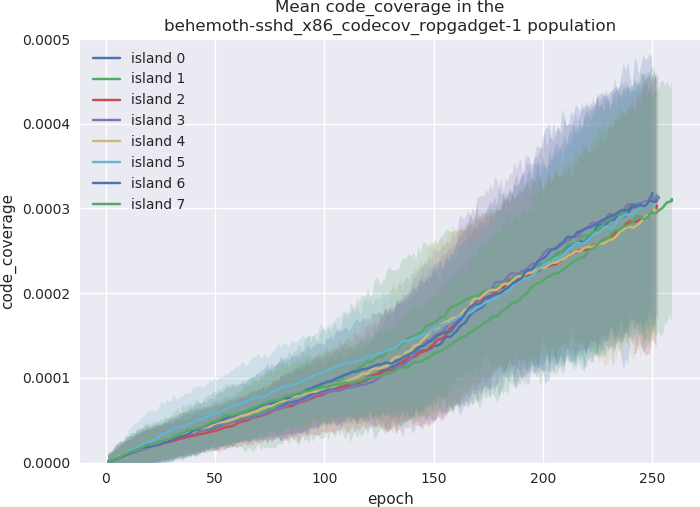
\includegraphics[align=c,width=0.42\textwidth]{cc/e2/6} \\
\end{tabular}
\end{center}
\caption{Code coverage of populations. Experiment 2.}
\label{fig:cc/e2}
\end{figure}

\begin{figure}[t]
\begin{center}
\begin{tabular}{c c c c}
    Seeding & Asexual reproduction & Alternating crossover & Fixed point crossover \\
    Random & 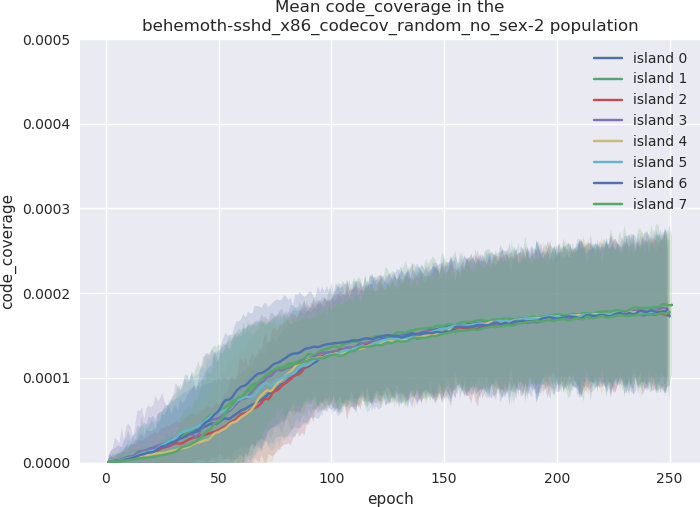
\includegraphics[align=c,width=0.42\textwidth]{cc/e3/1} & 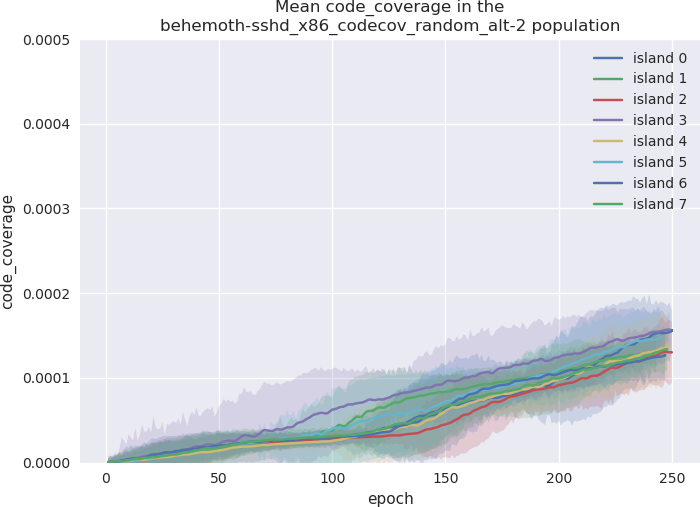
\includegraphics[align=c,width=0.42\textwidth]{cc/e3/2} & 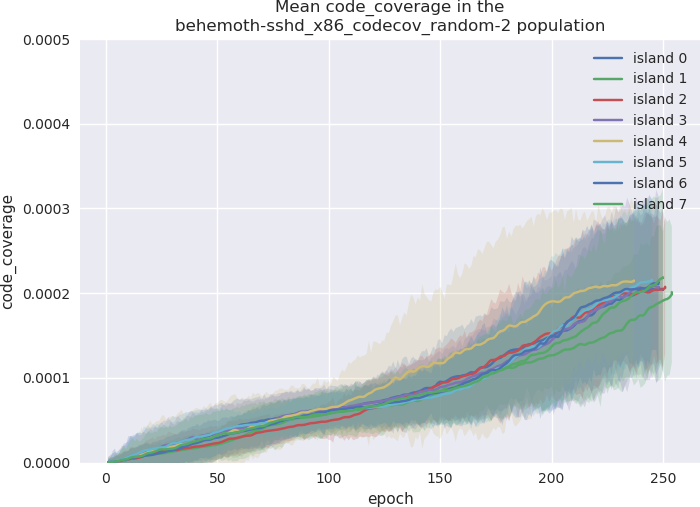
\includegraphics[align=c,width=0.42\textwidth]{cc/e3/3} \\
    & & & \\
    ROPgadget & 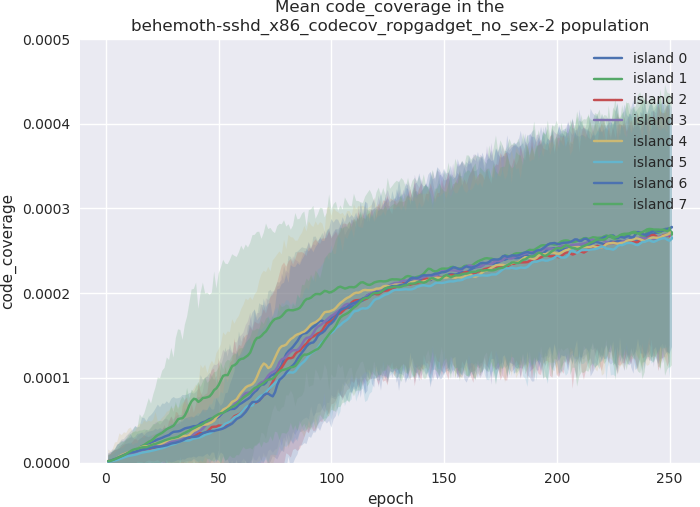
\includegraphics[align=c,width=0.42\textwidth]{cc/e3/4} & 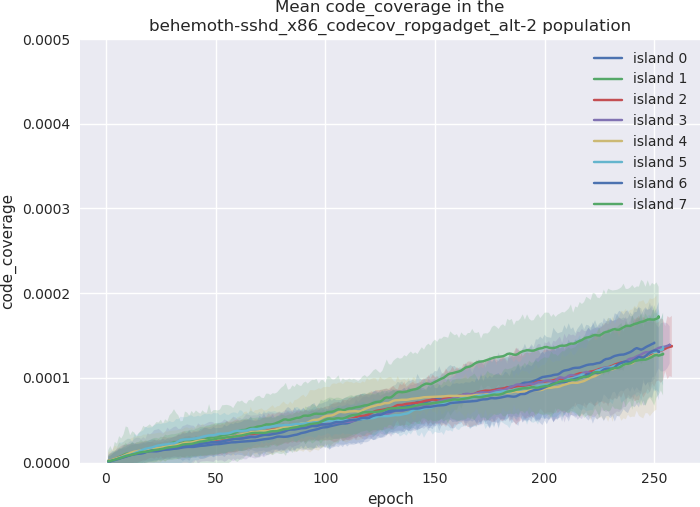
\includegraphics[align=c,width=0.42\textwidth]{cc/e3/5} & 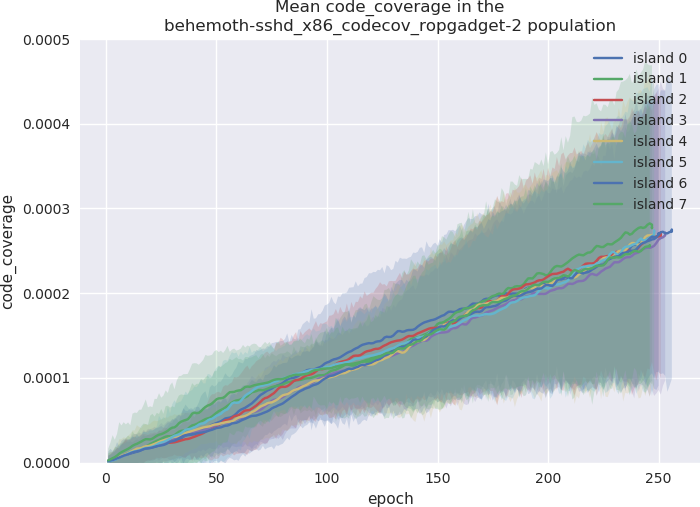
\includegraphics[align=c,width=0.42\textwidth]{cc/e3/6} \\
\end{tabular}
\end{center}
\caption{Code coverage of populations. Experiment 3.}
\label{fig:cc/e3}
\end{figure}
\end{landscape}
\restoregeometry
\pagestyle{plain}

\subsection{Allele circulation results}
A total of three experiments were run. In all of them, the cross product of reproduction and initial techniques were tested. The results of the experiments can be seen at figures \ref{fig:ac/e1}, \ref{fig:ac/e2} and \ref{fig:ac/e3}.

From the results in these figures, it is easy to notice that allele circulation was also maximized by single point crossover reproduction. As expected both crossover techniques also produced higher circulation than asexual reproduction since both parents could contribute their best alleles.

Using ROPgadget had only a significant effect on single point reproduction causing significantly higher number of allele occurrences in most cases. This may be likely caused by the ability of this technique of preserving and composing highly scoring contributions to a population member.


\newgeometry{top=5mm, bottom=5mm, right=5mm,left=5mm}
\pagestyle{empty}
\begin{landscape}
\begin{figure}[t]
\begin{center}
\begin{tabular}{c c c c}
    Seeding & Asexual reproduction & Alternating crossover & Single point crossover \\
    Random & 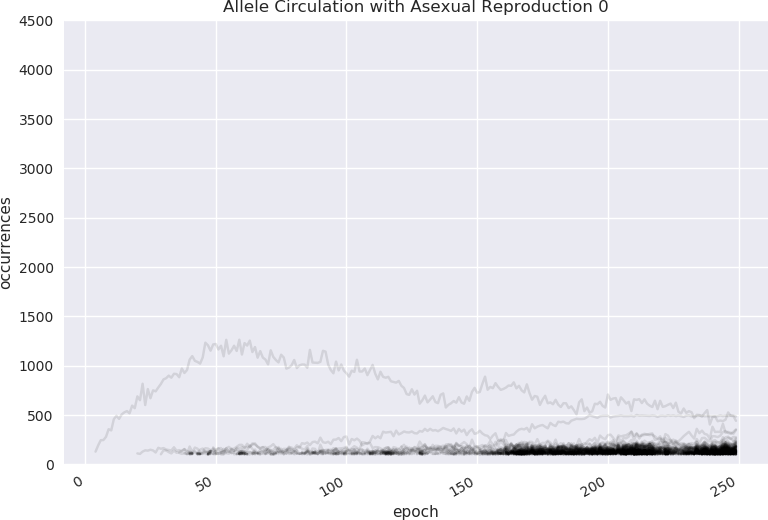
\includegraphics[align=c,width=0.42\textwidth]{ac/e1/1} & 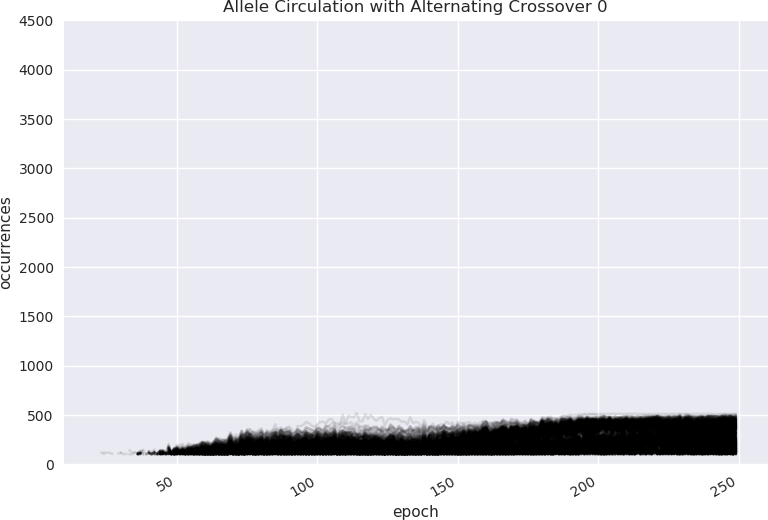
\includegraphics[align=c,width=0.42\textwidth]{ac/e1/2} & 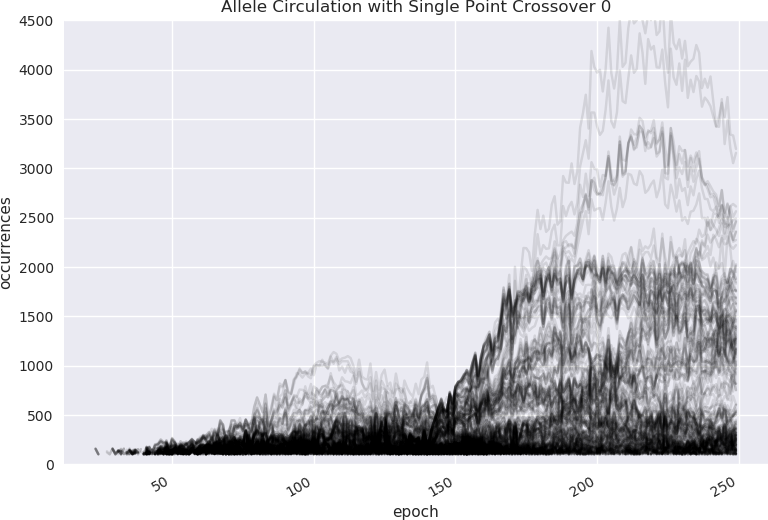
\includegraphics[align=c,width=0.42\textwidth]{ac/e1/3} \\
    & & & \\
    ROPgadget & 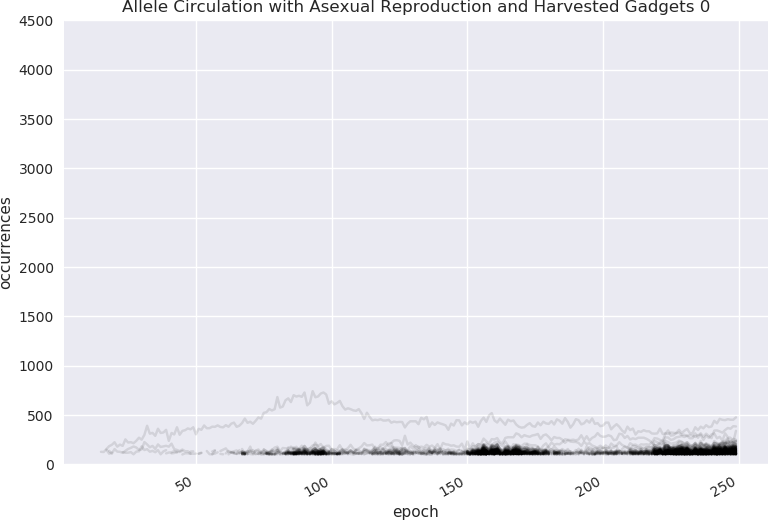
\includegraphics[align=c,width=0.42\textwidth]{ac/e1/4} & 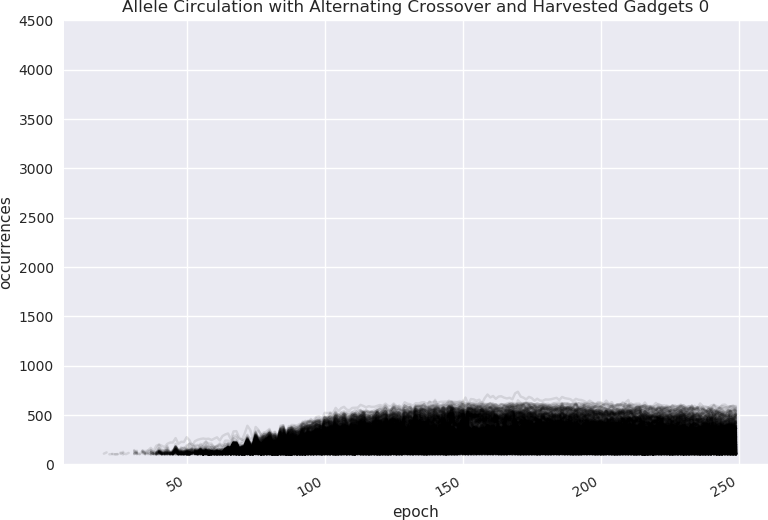
\includegraphics[align=c,width=0.42\textwidth]{ac/e1/5} & 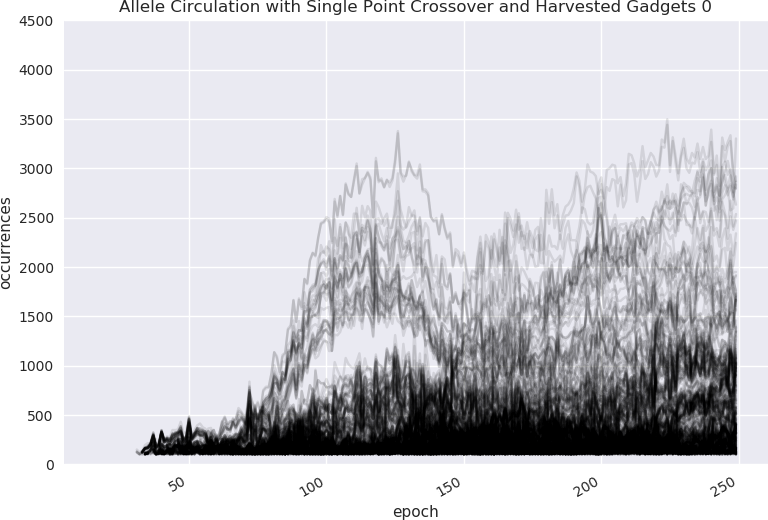
\includegraphics[align=c,width=0.42\textwidth]{ac/e1/6} \\
\end{tabular}
\end{center}
\caption{Allele circulation of populations. Experiment 1.}
\label{fig:ac/e1}
\end{figure}

\begin{figure}[t]
\begin{center}
\begin{tabular}{c c c c}
    Seeding & Asexual reproduction & Alternating crossover & Fixed point crossover \\
    Random & 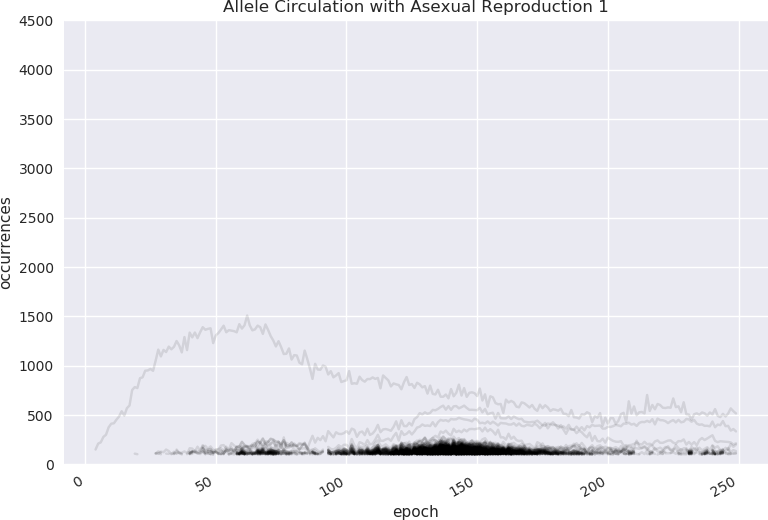
\includegraphics[align=c,width=0.42\textwidth]{ac/e2/1} & 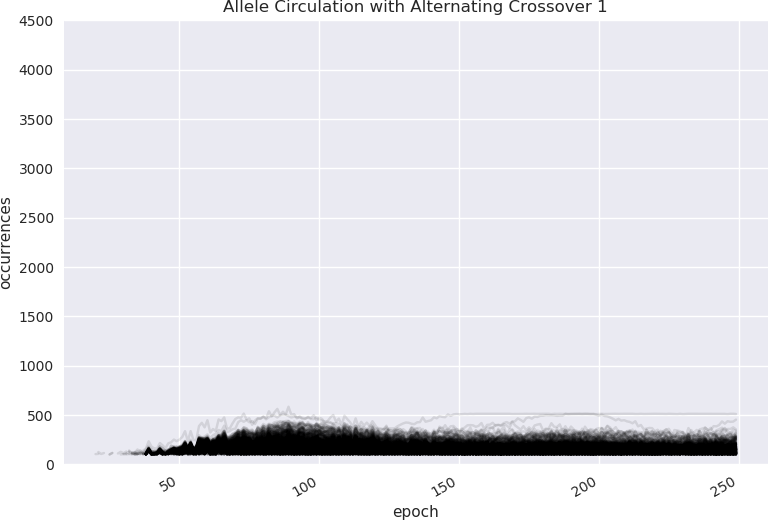
\includegraphics[align=c,width=0.42\textwidth]{ac/e2/2} & 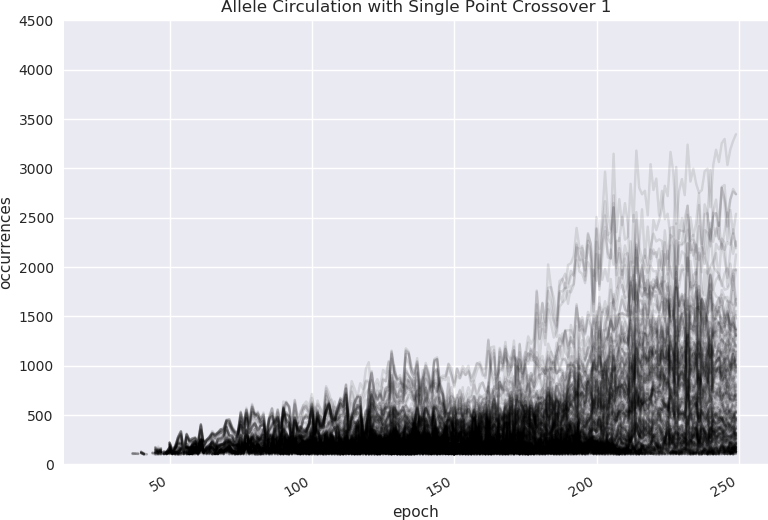
\includegraphics[align=c,width=0.42\textwidth]{ac/e2/3} \\
    & & & \\
    ROPgadget & \includegraphics[align=c,width=0.42\textwidth]{ac/e2/4} & \includegraphics[align=c,width=0.42\textwidth]{ac/e2/5} & \includegraphics[align=c,width=0.42\textwidth]{ac/e2/6} \\
\end{tabular}
\end{center}
\caption{Allele circulation of populations. Experiment 2.}
\label{fig:ac/e2}
\end{figure}

\begin{figure}[t]
\begin{center}
\begin{tabular}{c c c c}
    Seeding & Asexual reproduction & Alternating crossover & Fixed point crossover \\
    Random & \includegraphics[align=c,width=0.42\textwidth]{ac/e3/1} & \includegraphics[align=c,width=0.42\textwidth]{ac/e3/2} & \includegraphics[align=c,width=0.42\textwidth]{ac/e3/3} \\
    & & & \\
    ROPgadget & \includegraphics[align=c,width=0.42\textwidth]{ac/e3/4} & \includegraphics[align=c,width=0.42\textwidth]{ac/e3/5} & \includegraphics[align=c,width=0.42\textwidth]{ac/e3/6} \\
\end{tabular}
\end{center}
\caption{Allele circulation of populations. Experiment 3.}
\label{fig:ac/e3}
\end{figure}
\end{landscape}
\restoregeometry
\pagestyle{plain}

\subsection{Generational distribution results}
A total of three experiments were run. In all of them, the cross product of reproduction and initial techniques were tested. The results of the experiments can be seen at figures \ref{fig:gd/e1}, \ref{fig:gd/e2} and \ref{fig:gd/e3}.

From the results in these figures, it is easy to notice that generational distribution was also maximized by single point crossover reproduction. As expected both crossover techniques also had more successful children in later generations than asexual reproduction since both parents could contribute their best alleles.

Using ROPgadget had no signficant effects on the ability of individuals to survive over many generations. This is likely because all of the initial individuals start with similar genes and therefore have no significant advantage over the others.

\newgeometry{top=5mm, bottom=5mm, right=5mm,left=5mm}
\pagestyle{empty}
\begin{landscape}
\begin{figure}[t]
\begin{center}
\begin{tabular}{c c c c}
    Seeding & Asexual reproduction & Alternating crossover & Single point crossover \\
    Random & \includegraphics[align=c,width=0.42\textwidth]{gd/e1/1} & \includegraphics[align=c,width=0.42\textwidth]{gd/e1/2} & \includegraphics[align=c,width=0.42\textwidth]{gd/e1/3} \\
    & & & \\
    ROPgadget & \includegraphics[align=c,width=0.42\textwidth]{gd/e1/4} & \includegraphics[align=c,width=0.42\textwidth]{gd/e1/5} & \includegraphics[align=c,width=0.42\textwidth]{gd/e1/6} \\
\end{tabular}
\end{center}
\caption{Generational distribution of populations. Experiment 1.}
\label{fig:gd/e1}
\end{figure}

\begin{figure}[t]
\begin{center}
\begin{tabular}{c c c c}
    Seeding & Asexual reproduction & Alternating crossover & Fixed point crossover \\
    Random & \includegraphics[align=c,width=0.42\textwidth]{gd/e2/1} & \includegraphics[align=c,width=0.42\textwidth]{gd/e2/2} & \includegraphics[align=c,width=0.42\textwidth]{gd/e2/3} \\
    & & & \\
    ROPgadget & \includegraphics[align=c,width=0.42\textwidth]{gd/e2/4} & \includegraphics[align=c,width=0.42\textwidth]{gd/e2/5} & \includegraphics[align=c,width=0.42\textwidth]{gd/e2/6} \\
\end{tabular}
\end{center}
\caption{Generational distribution of populations. Experiment 2.}
\label{fig:gd/e2}
\end{figure}

\begin{figure}[t]
\begin{center}
\begin{tabular}{c c c c}
    Seeding & Asexual reproduction & Alternating crossover & Fixed point crossover \\
    Random & \includegraphics[align=c,width=0.42\textwidth]{gd/e3/1} & \includegraphics[align=c,width=0.42\textwidth]{gd/e3/2} & \includegraphics[align=c,width=0.42\textwidth]{gd/e3/3} \\
    & & & \\
    ROPgadget & \includegraphics[align=c,width=0.42\textwidth]{gd/e3/4} & \includegraphics[align=c,width=0.42\textwidth]{gd/e3/5} & \includegraphics[align=c,width=0.42\textwidth]{gd/e3/6} \\
\end{tabular}
\end{center}
\caption{Generational distribution of populations. Experiment 3.}
\label{fig:gd/e3}
\end{figure}
\end{landscape}
\restoregeometry
\pagestyle{plain}

\subsection{Experiment conclusions}
From these results we can see that single point crossover is the most promising of the reproduction techniques since it not only provides better solutions but does so faster. On the other hand, although slightly better, alternating crossover is not significantly better than asexual reproduction, specially over longer runs.

Regarding the use of ROPGadget, we can see that it does not speed up asexual reproduction significantly but is particularly useful when using single point crossover.

As for allele circulation we can notice it is fastest with single point crossover and slowest with alternating crossover.

Finally we can also notice that higher number of return instructions correlate with higher code coverage. Most likely because they allow to explore code across different functions that would not be reached otherwise.

\section{Register control}
A different target to show the effectiveness of Berbalang's techniques is by aiming for register control instead of code coverage. If the attacker has full control of the register contents, the attacker may not only perform calls to the operating system but also have the possibility of calling routines and procedures that are already in the system. This happens because parameters are frequently passed through a combination of registers and the stack in most architectures.

In our tests we attempted to reproduce control on an execve call by finding controlled targets with a mix of references and values for the eax, ebx, ecx and edx registers.

Unlike code coverage, scoring register control is significantly more difficult. On one hand, a graph with state transitions towards the solutions is too expensive to be useful; on the other, Euclidean and Hamming distance from the desired results are both too inaccurate to be meaningful. This also raises the questions on how to handle indirections and writable memory.

Berbalang tried instead to use an approach based on weighted hamming distances. For each register and the first m references in memory, the closest target was chosen and then 1 point was added for each disagreement. An additional penalty was also applied if the result was found on a different register. Finally the sum of all the results gave the distance used to score the fitness of the individuals.

Despite these efforts, solutions offering full register control were found to be very rare. Only 20\% of the trials made up to 1000 generations resulted in solutions. To improve the results it was necessary to apply secondary novelty pressure. To do so, count-min-sketch was used to weight errors so that new errors had a smaller impact on the score than existing ones. This allowed possible mutations that did not have a direct improvement but that would later lead to a different solution to remain.

In our testing we also found that the push VM did not prove to be a better representation than ROP Chains were when finding solutions. The solutions that were found can be seen on figures \ref{fig:rc1} and \ref{fig:rc2}.

\begin{figure}[ht]
\centering
\begin{verbatim}
#+CAPTION: Champion of a system call preparation trial
#+NAME: ex:champion-1
#+BEGIN_EXAMPLE

Name: wiles-flied-nooks-whipt, from island 0
Generation: 2736

Trace:
----
80b5dfa:	 89 f0                mov eax, esi
80b5dfc:	 8b 4c 24 54          mov ecx, dword ptr [esp + 0x54]
80b5e00:	 25 00 00 00 c0       and eax, 0xc0000000
80b5e05:	 01 c1                add ecx, eax
80b5e07:	 03 44 24 58          add eax, dword ptr [esp + 0x58]
80b5e0b:	 81 e6 ff ff ff 3f    and esi, 0x3fffffff
80b5e11:	 89 c2                mov edx, eax
80b5e13:	 74 39                je 0x80b5e4e
----
80b5e4e:	 83 c4 3c             add esp, 0x3c
80b5e51:	 b8 01 00 00 00       mov eax, 1
80b5e56:	 5b                   pop ebx
80b5e57:	 5e                   pop esi
80b5e58:	 5f                   pop edi
80b5e59:	 5d                   pop ebp
80b5e5a:	 c3                   ret 
----
8075df7:	 52                   push edx
8075df8:	 1c f6                sbb al, 0xf6
8075dfa:	 c2 02 74             ret 0x7402


Spidered register state:
EAX: 0xb
EBP: 0x81606d5 RX -> 0x312e2520 " %.1"
EBX: 0x81606a8 RX -> 0x6e69622f "/bin"
ECX: 0x8049633 RX -> 0x0
EDX: 0x0
EIP: 0x8075dfa RX -> 0xe7402c2
ESP: 0x8218150 RW (stack) -> 0x0
#+END_EXAMPLE
\end{verbatim}
\caption{First solution to the register control problem.}
\label{fig:rc1}
\end{figure}

\begin{figure}[ht]
\centering
\begin{verbatim}
#+CAPTION: Another champion of the system call preparation task
#+NAME: ex:champion-2
#+BEGIN_EXAMPLE
Name: corms-taxis-magma-wefts, from island 4
Generation: 951

Trace:
----
80badf1:	 83 fb ff             cmp ebx, -1
80badf4:	 74 0f                je 0x80bae05
80badf6:	 8d 4b 10             lea ecx, [ebx + 0x10]
80badf9:	 31 d2                xor edx, edx
80badfb:	 39 4c 24 5c          cmp dword ptr [esp + 0x5c], ecx
80badff:	 0f 85 99 01 00 00    jne 0x80baf9e
80baf9e:	 83 c4 3c             add esp, 0x3c
80bafa1:	 89 d0                mov eax, edx
80bafa3:	 5b                   pop ebx
80bafa4:	 5e                   pop esi
80bafa5:	 5f                   pop edi
80bafa6:	 5d                   pop ebp
80bafa7:	 c3                   ret 
----
80badf1:	 83 fb ff             cmp ebx, -1
80badf4:	 74 0f                je 0x80bae05
80badf6:	 8d 4b 10             lea ecx, [ebx + 0x10]
80badf9:	 31 d2                xor edx, edx
80badfb:	 39 4c 24 5c          cmp dword ptr [esp + 0x5c], ecx
80badff:	 0f 85 99 01 00 00    jne 0x80baf9e
80baf9e:	 83 c4 3c             add esp, 0x3c
80bafa1:	 89 d0                mov eax, edx
80bafa3:	 5b                   pop ebx
80bafa4:	 5e                   pop esi
80bafa5:	 5f                   pop edi
80bafa6:	 5d                   pop ebp
80bafa7:	 c3                   ret 
\end{verbatim}
\caption{Second solution to the register control problem. First part.}
\label{fig:rc2}
\end{figure}
\begin{figure}[ht]
\ContinuedFloat
\centering
\begin{verbatim}
----
80badf1:	 83 fb ff             cmp ebx, -1
80badf4:	 74 0f                je 0x80bae05
80badf6:	 8d 4b 10             lea ecx, [ebx + 0x10]
80badf9:	 31 d2                xor edx, edx
80badfb:	 39 4c 24 5c          cmp dword ptr [esp + 0x5c], ecx
80badff:	 0f 85 99 01 00 00    jne 0x80baf9e
80baf9e:	 83 c4 3c             add esp, 0x3c
80bafa1:	 89 d0                mov eax, edx
80bafa3:	 5b                   pop ebx
80bafa4:	 5e                   pop esi
80bafa5:	 5f                   pop edi
80bafa6:	 5d                   pop ebp
80bafa7:	 c3                   ret 
----
8088fa1:	 7d 94                jge 0x8088f37
8088f37:	 ac                   lodsb al, byte ptr [esi]
8088f38:	 c3                   ret 


Spidered register state:
EAX: 0xb
EBP: 0x81e9182 RX -> 0xe00c0002
EBX: 0x8189e76 RX -> 0x6e69622f "/bin"
ECX: 0x80482dd RX -> 0x0
EDX: 0x0
EIP: 0x8088f38 RX -> 0xf13101c3
ESP: 0x82181f4 RW (stack) -> 0x80ad3ae RX -> 0x8b097400

#+END_EXAMPLE
\end{verbatim}
\caption{Second solution to the register control problem. Second part.}
\label{fig:rc2_cont}
\end{figure}

\clearpage
\section{Current project status}

\subsection{Berbalang}
During development we found that Rust significantly slowed down experimentation as it required compiling a full new version of Berbalang every time. While the performance benefits from slower compilation might outweigh the compilation time when running many experiments in parallel or running them for longer periods of time, we found that this overhead was unacceptable when testing different approaches to the problem.

Additionally, we found that Rust lacks a good way of allowing task distribution across processors and systems which is critical when scaling the experiments over clusters.

Because of these limitations, work has started on a next iteration of Berbalang using Julia. This will allow avoiding the need to use Linux containers and lxd, allow to easily distribute execution using ssh and make modifications easier.

\subsection{Mario project}
Our team has started working on using reinforcement learning in order to generalize the techniques learned from this project to different systems.

For this approach we use a simulator able to perform various runs of the Super Mario Bros 3 game in parallel. The runs are already on a weird state commonly used by speed runners and which may allow certain inputs to lead to execution of unintended code. This approach increases the complexity of the candidates since inputs also depend on the time (in frames) when they are performed. For scoring we are also considering the ability of the runs to cover the address space of the system.

At this stage it is too early to draw conclusions from this approach but results seem promising. Some screenshots of the application at play with different interesting results can be seen in figures \ref{fig:ma1}, \ref{fig:ma2} and \ref{fig:ma3}.

\begin{figure}[ht]
\centering
\includegraphics[width=\textwidth]{ma1}
\caption{A run of the Mario project}
\label{fig:ma1}
\end{figure}

\begin{figure}[ht]
\centering
\includegraphics[width=\textwidth]{ma2}
\caption{Another run of the Mario project}
\label{fig:ma2}
\end{figure}

\begin{figure}[ht]
\centering
\includegraphics[width=\textwidth]{ma3}
\caption{A third run of the Mario project}
\label{fig:ma3}
\end{figure}

\subsection{Public resources}
\begin{itemize}
    \item The october report is publicly available at \url{https://github.com/oblivia-simplex/berbalang/blob/master/org/october_report.org}
    \item The Berbalang source code is available at \url{https://github.com/oblivia-simplex/berbalang}
    \item Our Unicorn patches are available at \url{https://github.com/oblivia-simple/unicorn-rs}
    \item The bindings to make Unicorn work on Julia are available on \url{https://github.com/oblivia-simplex/unicorn-jl}
\end{itemize}

\section{Future directions}
Currently the main project efforts are on the Mario project and the final project report will be made somewhere in April.

Regarding Berbalang, the project will likely continue if further funding is found. There are still many avenues that have been untested.

One of the team members is planning to try to use it as a way to generate a measure of the level of control an attacker can have by using already existing code. If successful this may result in a research paper being published in June.

\end{document}
